%
%  untitled
%
%  Created by Hidde-Jan Jongsma on 2010-10-22.
%  Copyright (c) 2010 __MyCompanyName__. All rights reserved.
%
\documentclass[]{beamer}

% Use utf-8 encoding for foreign characters
\usepackage[utf8]{inputenc}

\usetheme{Malmoe}


% Setup for fullpage use
% \usepackage{fullpage}

% Uncomment some of the following if you use the features
%
% Running Headers and footers
%\usepackage{fancyhdr}

% Multipart figures
%\usepackage{subfigure}

% More symbols
\usepackage{amsmath}
\usepackage{amssymb}
\usepackage{latexsym}

\usepackage{mathtools}

% Surround parts of graphics with box
\usepackage{boxedminipage}

% Package for including code in the document
\usepackage{listings}

% If you want to generate a toc for each chapter (use with book)
% \usepackage{minitoc}

% This is now the recommended way for checking for PDFLaTeX:
%\usepackage{ifpdf}
%
%\newcommand{\e}{\epsilon}
%\newcommand{\s}{\sigma}
%\newcommand{\be}{\beta}
%\newcommand{\g}{\gamma}
%\newcommand{\om}{\omega}
%\newcommand{\T}{\mathbb{T}}
%\newcommand{\KAM}{KAM  }
%\newcommand{\rst}{\! \mid}

% Create graphics in LaTex
\usepackage{tikz}

% Extra commands
\newcommand{\Reals}{\mathbb{R}}

\newcommand{\dd}{\mathrm{d}}

\newcommand{\dun}{\frac{\partial u}{\partial n}}
\newcommand{\dux}{\frac{\partial u}{\partial x}}
\newcommand{\duxx}{\frac{\partial^2 u}{\partial x^2}}
\newcommand{\duxxx}{\frac{\partial^3 u}{\partial x^3}}

\newcommand{\duy}{\frac{\partial u}{\partial y}}
\newcommand{\duyy}{\frac{\partial^2 u}{\partial y^2}}
\newcommand{\duyyy}{\frac{\partial^3 u}{\partial y^3}}
\newcommand{\lapu}{\nabla^2 u}

\newcommand{\vct}{}

\providecommand{\abs}[1]{\lvert#1\rvert}
\providecommand{\norm}[1]{\lVert#1\rVert}

\newcommand{\LO}{\ensuremath{L_2(\Omega)}}
\newcommand{\HO}{\ensuremath{H^1(\Omega)}}
\newcommand{\HOzero}{\ensuremath{H^1_{(0}(\Omega)}}

%\newif\ifpdf
%\ifx\pdfoutput\undefined
%\pdffalse % we are not running PDFLaTeX
%\else
%\pdfoutput=1 % we are running PDFLaTeX
%\pdftrue
%\fi

% \ifpdf
% \usepackage[pdftex]{graphicx}
% \else
% \usepackage{graphicx}
% \fi
\title{Finite Difference and Finite Element Methods \\ for Helmholtz scattering problems}
\author{ Hidde-Jan Jongsma }
\institute{ RuG }

\date{\today}

\begin{document}

% \ifpdf
% \DeclareGraphicsExtensions{.pdf, .jpg, .tif}
% \else
% \DeclareGraphicsExtensions{.eps, .jpg}
% \fi

\maketitle

\section{Introduction}

\begin{frame}{Outline}
    \small \tableofcontents
\end{frame}

\subsection{What is FDM/FEM?}

\begin{frame}{What is FDM/FEM?}
  Frequently used for acoustic electromagnetic scattering problems.

  Approach:
    \begin{itemize}
        \item Discretize domain $\Omega$.
        \item Create new constraints that mimic `real' ones.
        \item Find solution to these constrains that \emph{approximate} the exact solution.
    \end{itemize}
  
  Unbounded domains or complex geometries $\rightarrow$ use FEM.
\end{frame}

\begin{frame}{Helmholtz equations}
    \begin{definition}
      The Helmholtz equations are given by
\begin{align}
  \Delta u + k^2 u & = 0, \quad \text{in}\ \Omega, \label{eq:Duku} \\
  \frac{\partial u}{\partial n} + \beta u & = g, \quad \text{on}\ \Gamma, \label{eq:2Dbc}
\end{align}
      for $u : \Omega \rightarrow \Reals$.
    \end{definition}
    
\end{frame}

\section{Finite difference method}

\subsection{Finite difference method}

\begin{frame}{Finite difference method}
    
  \begin{itemize}
    \item Grid on domain $\Omega \subseteq \Reals^d, d = 1, 2, 3$.
    \item Approximate $\nabla^2 u$ by finite difference.
  \end{itemize}

  \begin{equation*}
    \nabla^2 u + f u = g, \text{ on } \Omega.
  \end{equation*}
    
  Grid on 1D $\Omega = (0, 1)$:
\begin{equation*}
  X_h = \left\{ x_i\ |\ x_i = h i,\ i = 0, 1, \ldots, N \right\}
\end{equation*}

\end{frame}

\subsection{Finite difference}

\begin{frame}{Finite difference}

We define $u_i = u(x_i)$. Use Taylor series to approximate $\dd^2 u / \dd x^2$:
\begin{align}
  u_{i + 1} & = u_{i} + h \frac{\dd u}{\dd x}
    + \frac{h^2}{2} \frac{\dd^2 u}{\dd x^2}
    + \frac{h^3}{6} \frac{\dd^3 u}{\dd x^3}
    + \frac{h^4}{24} \frac{\dd^4 u}{\dd x^4} 
    + \mathcal{O}(h^5) \\
%
  u_{i - 1} & = u_{i} - h \frac{\dd u}{\dd x}
    + \frac{h^2}{2} \frac{\dd^2 u}{\dd x^2}
    - \frac{h^3}{6} \frac{\dd^3 u}{\dd x^3}
    + \frac{h^4}{24} \frac{\dd^4 u}{\dd x^4}
    + \mathcal{O}(h^5).
\end{align}
This results in
\begin{equation}
  \frac{\dd^2 u}{\dd x^2}(x_i)
  \approx
    \frac{1}{h^2} \left[ u_{i + 1} - 2 u_i + u_{i - 1} \right],
\end{equation}
which has a truncation error of the form $ - \frac{h^2}{12} \frac{\dd^4 u}{\dd x^4}(x_i)$.

\end{frame}

\subsection{Five-point formula}

\begin{frame}{Five-point formula}

\begin{columns}[c]
\column{.5\textwidth}

For two dimensions, the commonly used form is the
\emph{five-point formula}.
\begin{align*}
  \nabla^2 u(x, y) & \approx \\ &  \frac{1}{h^2} ( 
      u(x + h, y) + u(x - h, y) \\ & + u(x, y + h)
      + u(x, y - h) \\ & - 4 u(x, y) ).
\end{align*}

\column{.5\textwidth}
\begin{figure}
    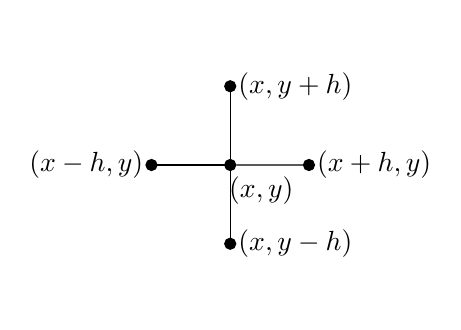
\begin{tikzpicture}
    \tikzstyle{every node}=[draw,circle,fill=black,minimum size=4pt,
                            inner sep=0pt]

      \draw (0,0) node (0) [label=left:${(x - h, y)}$] {}
        -- ++(0:1.0cm) node (1) [label=-5:${(x, y)}$] {}
        -- ++(90:1.0cm) node (2) [label=right:${(x, y + h)}$] {} 
        ++(-90:2.0cm) node (3) [label=right:${(x, y - h)}$] {}
        ++(45:1.414213cm) node (4) [label=right:${(x + h, y)}$] {};

      \draw (1) -- (3);
      \draw (1) -- (4);
    \end{tikzpicture}
    \caption{Five-point stencil}
\end{figure}
\end{columns}

\end{frame}

\section{Finite element method}
\subsection{Finite element method}

\begin{frame}{Finite element method}

\begin{itemize}
  \item Approximate solution to weak form of problem.
  \item Uses search space of functions defined on set of \emph{finite elements}.
\end{itemize}

\begin{definition}
  $f \in \LO$:
  \begin{equation*}
  \lVert f \rVert := \left(
    \int_\Omega | f(x) |^2 \ \dd\Omega \right)^{\frac{1}{2}} < \infty.
  \end{equation*}
  $f \in \HO$:
\begin{equation*}
  \lVert \nabla f \rVert^2 + \lVert f \rVert^2 < \infty.
\end{equation*}
  $f \in \HOzero$ if $f \in \HO$ and $f(0) = 0$.
\end{definition}
\end{frame}

\subsection{Weak formulation}

\begin{frame}{Weak formulation}
The weak form of the problem is given by 
\begin{equation*}
  - \int^1_0 u''(x)v(x) - k^2u(x)v(x) \ \dd x = \int^1_0 f(x)v(x) \ \dd x,
\end{equation*}
where $v \in \HOzero$. We integrate the first term by parts to get
\begin{equation*} \label{eq:weakprob}
  \int^1_0 u'(x)v'(x)\ \dd x - k^2 \int^1_0 u(x)v(x) \ \dd x - iku(1)v(1) = \int^1_0 f(x)v(x) \ \dd x.
\end{equation*}
\end{frame}

\subsection{Basis functions}

\begin{frame}{Basis functions}
We refine ours search space to the piecewise linear function $S_h(0, 1)$.

This is spanned by the \emph{basis functions}, $j = 1, \ldots, N - 1$
\begin{equation*}
  \chi_j(x) = \begin{dcases*}
    \frac{1}{h} (x - x_{j - 1}), & $x \in [x_{j - 1}, x_j],$ \\
    \frac{1}{h} (x_{j + 1} - x), & $x \in [x_{j}, x_{j + 1}],$ \\
    0 & elsewhere,
  \end{dcases*}, \quad
\end{equation*}
\begin{equation*}
  \chi_N(x) = \begin{dcases*}
    \frac{1}{h} (x - x_{j - 1}), & $x \in [x_{j - 1}, 1],$ \\
    0 & elsewhere.
  \end{dcases*}
\end{equation*}
\end{frame}

\subsection{Approximation}

\begin{frame}{Approximation}
  We require $U(x) \in S_h(0, 1)$, we can write
  \begin{equation*}
    U(x) = \sum_{j = 1}^N u_j \chi_j(x).
  \end{equation*}

  Our problem reduces to:
\begin{equation*} \label{eq:linsys}
  \begin{split}
  \sum^N_{j = 1} \left[ \int^1_0 \chi_j'(x) \chi_m'(x) \ \dd x
    - k^2 \int^1_0 \chi_j(x) \chi_m(x) \ \dd x \right] u_j
    - i k u_N \chi_m(1)
 \\ =
    \int^1_0 f(x) \chi_m(x) \ \dd x,
    \end{split}
\end{equation*}
for $m = 1, 2, \ldots, N$.
\end{frame}

\subsection{Linear system}

\begin{frame}{Linear system}
  This gives rise to a linear system of the form
  \begin{equation*}
    (A - k^2 B - i k C)u = f,
  \end{equation*}
  where
\begin{equation*}
  A_{i j} = \int^1_0 \chi_i'(x) \chi_j'(x) \ \dd x, \quad
  B_{i j} = \int^1_0 \chi_i(x) \chi_j(x) \ \dd x.
\end{equation*}
\end{frame}

\begin{frame}
\begin{equation*}
  A = \begin{pmatrix}
        \frac{2}{h}   & - \frac{1}{h} & 0             & \hdots        & 0             \\
        - \frac{1}{h} & \frac{2}{h}   & - \frac{1}{h} &  \ddots       & \vdots        \\
        0             & - \frac{1}{h} & \frac{2}{h}   & \ddots        & 0             \\
        \vdots        & \ddots        & \ddots        & \ddots        & - \frac{1}{h} \\
        0             & \hdots        & 0             & - \frac{1}{h} & \frac{1}{h}
      \end{pmatrix},
  \quad
  B = \begin{pmatrix}
        \frac{2h}{3}  & \frac{h}{6}   & 0             & \hdots      & 0           \\
        \frac{h}{6}   & \frac{2h}{3}  & \frac{h}{6}   & \ddots      & \vdots      \\
        0             & \frac{h}{6}   & \frac{2h}{3}  & \ddots      & 0           \\
        \vdots        & \ddots        & \ddots        & \ddots      & \frac{h}{6} \\
        0             & \hdots        & 0             & \frac{h}{6} & \frac{h}{3}
      \end{pmatrix},
\end{equation*}
\begin{equation*}
  C = \begin{pmatrix}
        0       & 0       & \hdots  & 0       \\
        0       & 0       & \ddots  & \vdots  \\
        \vdots  & \ddots  & \ddots  & 0       \\
        0       & \hdots  & 0       & 1
      \end{pmatrix},
  \quad
  \vct{u} = \begin{pmatrix}
              u_1 \\
              u_2 \\
              \vdots \\
              u_N
            \end{pmatrix},
  \quad
  \vct{f} = \begin{pmatrix}
              \int^1_0 f(x) \chi_1(x) \ \dd x \\
              \int^1_0 f(x) \chi_2(x) \ \dd x \\
              \vdots \\
              \int^1_0 f(x) \chi_N(x) \ \dd x \\
            \end{pmatrix}.
\end{equation*}

Matrix $(A - k^2 B - i k C)$ is \emph{sparse}, \emph{tridiagonal}. 
\end{frame}

\section{Difficulties and pitfalls}
\subsection{Difficulties and pitfalls}
\begin{frame}{Difficulties and pitfalls}
Error estimate
\begin{equation*} \label{eq:ErrEst}
  \frac{\lVert u - U \rVert}{\lVert u \rVert} \leq C_1 k h + C_2 k^3
  h^2,
\end{equation*}
where $C_1$, $C_2$ independent of $k, h$.

\medskip
\begin{center}
  
\emph{Higher wavenumber} $\rightarrow$ \emph{smaller mesh size}.
\end{center}
\medskip
Size of linear system grows very rapidly, as does the \emph{bandwidth}
of the system matrix.
\end{frame}

\subsection{Higher order problem}
\begin{frame}{Higher order problem}
  \begin{itemize}
    \item Mesh generation non-trivial (Delaunay triangulation).
    \item Rapidly growing linear system.
    \item Higher wavenumber means more computational effort.
  \end{itemize}

  Remedy: order of piece wise polynomial search space functions.

  \medskip
  Special boundary conditions for unbounded domains: \emph{absorbent boundary condition},
  \emph{non-reflecting boundary condition}.
\end{frame}

\section{Conclusion}

\subsection{Conclusion}

\begin{frame}{Conclusion}
  \begin{itemize}
    \item FDM is still used, but FEM is more flexible.
    \item If the whole domain is important $\rightarrow$ use FEM.
    \item Unbounded domains can be tackled using special BC's.
    \item Sparse matrices with low bandwidth.
  \end{itemize}

  If you have an unbounded domain and are only interested in surface of
  an object: use BEM.
\end{frame}

\begin{frame}
\begin{center}
  {\Large Thank you for listening}
\end{center}
\end{frame}
%\bibliographystyle{plain}
%\bibliography{}
\end{document}
